\documentclass{beamer}
\usepackage{amsmath}
\usepackage{stmaryrd}
\usepackage{proof}
\usepackage{array}
\usepackage{pb-diagram}
\usepackage{graphicx}
\usepackage{centernot}

% Beamer appearance
\usepackage{helvet}
\definecolor{MaltaBlue}{RGB}{81,118,147}
\definecolor{FireBrick}{RGB}{228,34,23}
\setbeamertemplate{navigation symbols}{}
\setbeamertemplate{headline}{} % removes navtree
\setbeamercolor{example text}{fg=MaltaBlue}
\setbeamercolor{footline}{fg=MaltaBlue}
\setbeamercolor{structure}{fg=MaltaBlue}
\setbeamercolor{alerted text}{fg=FireBrick}
\setbeamertemplate{footline}{\strut\hfill%
\insertframenumber/\inserttotalframenumber~~}

\AtBeginSection[]
{
\begin{frame}{}
\centerline{\Large \textcolor{MaltaBlue}{\insertsectionhead}}
\end{frame}
} 

%%%%%%%%%%%%%%%%%%%%%%%%%%%%%%%%%%%%%%%%%%%%%%%%%%%%%%%%%%%%%%%%%%%%%%%%%%%%%%%%

\title{%
\texorpdfstring{%
\only<1>{Excise Implementations for \\ Deductive Rule Schemata}%
\only<2>{Monetizing Free-to-Play Logics \\ ~}%
}{Monetizing Free-to-Play Logics}
}
\author{Carlo Angiuli}
\date{April 1, 2014}
\institute{Carnegie Mellon University}

\newcommand{\coin}{
\includegraphics[width=.7em]{coin.png}}
\newcommand{\tophat}[1]{\ensuremath{\overset{\raisebox{-1.4em}[-1em]{
\includegraphics[width=.7em]{../images/tophat.png}}}{#1}}}
\newcommand{\sunhat}[1]{\ensuremath{\overset{\raisebox{-1.4em}[-1em]{
\includegraphics[width=.7em]{../images/sunhat.png}}}{#1}}}
\newcommand{\gradhat}[1]{\ensuremath{\overset{\raisebox{-1.4em}[-1em]{
\includegraphics[width=.7em]{../images/mortarboard.png}}}{#1}}}

\begin{document}

%%%%%%%%%%%%%%%%%%%%%%%%%%%%%%%%%%%%%%%%%%%%%%%%%%%%%%%%%%%%%%%%%%%%%%%%%%%%%%%%

\begin{frame}
\maketitle
\end{frame}

% most logics are given away for free! (to build reputation)
% or one-time purchase from Springer
\begin{frame}
\frametitle{A new revenue stream for logicians}
Designing logics is hard work.
\vspace{1em}

More users \alert{$\centernot\implies$} more money.
\end{frame}

\begin{frame}
\frametitle{A new revenue stream for logicians}
Turn each proof into a source of \alert{ongoing revenue}!
\end{frame}

% here are a couple weird tricks
\begin{frame}
\frametitle{Banner advertisements}
\[\deduce
  {\Delta\vdash A\otimes B}
  {\deduce
    {
\includegraphics[height=2.5em]{shirtad_whale.png}}
    {\Delta\vdash A & \Delta\vdash B}}
\]
\end{frame}

\begin{frame}
\frametitle{Resource interpretation}
Propositions as prover's resources.
\vspace{1em}

\[\infer[(\coin L)]
  {\Delta,\coin,\coin\vdash A}
  {\Delta\vdash A & \$1}
\]
\pause
\[\infer[(\coin CC)]
  {\Delta\vdash !\coin}
  {\text{Credit Card}}
\]
\end{frame}

% now, people don't like when content is hidden behind a paywall
% (also prohibits coin |- A)
\begin{frame}
\frametitle{Coin admissibility}
\begin{theorem}
If $\Delta,\coin\vdash A$ is derivable, then $\Delta\vdash A$ is derivable (for
$A\neq\coin$).
\end{theorem}
\end{frame}

% but it doesn't have to be easy.
% notice that the coin is consumed.
\begin{frame}
\frametitle{Premium admissible rules}
\[\infer[cut]
  {\Delta,\Delta'\vdash C}
  {\Delta\vdash A & \Delta',\only<2>{\coin,}A\vdash C}
\]
\end{frame}

\section{Alternate revenue sources}

% other premium content:
\begin{frame}
\frametitle{Decorative hats}
\[\infer
  {\Delta\vdash\widehat{A}}
  {\Delta,\coin\vdash A}
\]
\pause
\[\infer
  {\Delta\vdash\tophat{A}}
  {\Delta,\coin,\coin\vdash A}
\qquad
  \infer
  {\Delta\vdash\sunhat{A}}
  {\Delta,\coin,\coin\vdash A}
\qquad
  \infer
  {\Delta\vdash\gradhat{A}}
  {\Delta,\coin,\coin\vdash A}
\]
\end{frame}

% add features that might interest players of other popular games
% tensor-crush explodes the sequent if you have five copies of something
\begin{frame}
\frametitle{Tensor Crush Sequent}
\[\infer[(\otimes C)]
  {\ }
  {\Delta\vdash A\otimes A\otimes A\otimes A\otimes A}
\]
\end{frame}

% logic too hard?
\begin{frame}
\frametitle{Sell strategy guides}

\includegraphics[height=15em]{hott.png}\qquad
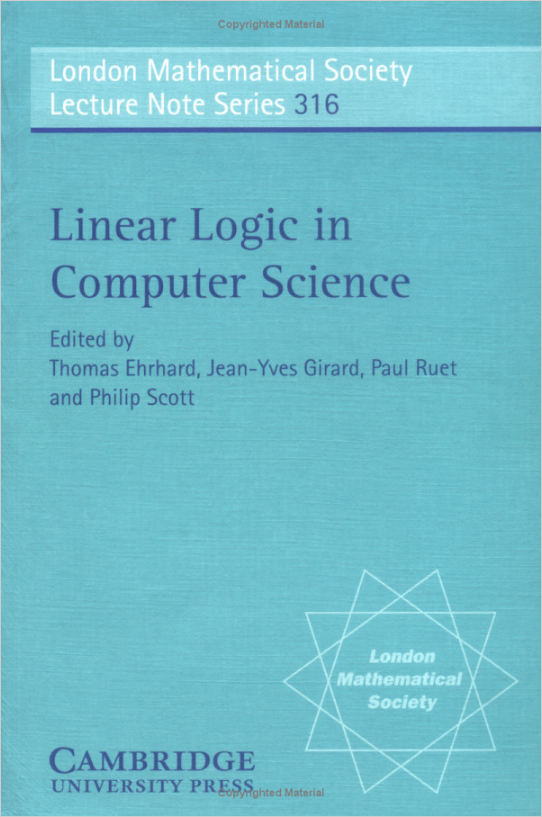
\includegraphics[height=15em]{linearlogic.png}
\end{frame}

\begin{frame}
\begin{center}

\includegraphics[width=18em]{appstore.png}
\end{center}
\end{frame}

\end{document}
